Interfejs graficzny jest tworzony przez Django. Django na podstawie szablonów w postaci plików html oraz danych otrzymanych z funkcji napisanych w python'ie przygotowuje kompletny podgląd strony. 
Strona główna (Rysunek \ref{fig:stronaStartowa}) składa się z 3 dużych przycisków animowanych przy użyciu javascript, które doprowadzają do kolejnych zakładek. W górnej części strony znajdują się przyciski (''Indeks'', ''Podgląd stacji pogodowych'', ''Prognoza'', \textit{''Wczytaj dane''}, ''Autorzy''). W przypadku przycisku ''Wczytaj dane'' nie pojawi się on jeśli użytkownik jest niezalogowany. \newline 
\begin{figure}[p]
	\centering
	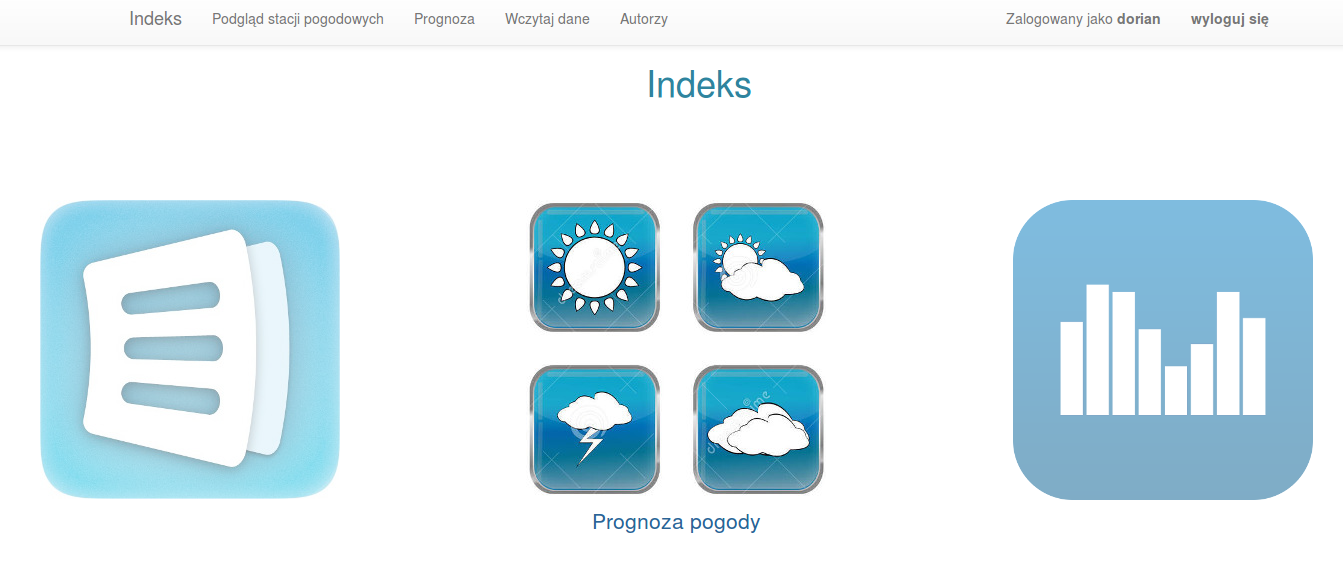
\includegraphics[width=\textheight, angle=90]{000}
	\caption{Strona startowa}
	\label{fig:stronaStartowa}
	\end{figure}

Po kliknięciu na zakładki ''Podgląd stacji pogodowych'' oraz ''Prognoza'' otwiera się bardzo podobna podstrona (Rysunek \ref{fig:podgladStacji}), która służy do wyboru rodzaju pomiaru oraz stacji, dla której dane mają zostać wyrysowane. W przypadku zalogowanych użytkowników pojawia się również możliwość skasowania danych w postaci przycisku ''delete''. 
\newline
\begin{figure}[p]
	\centering
	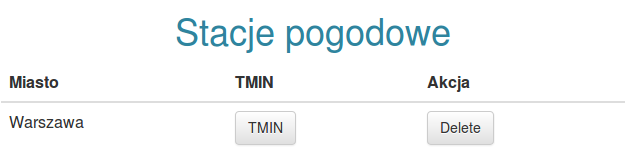
\includegraphics[width=\linewidth]{001}
	\caption{Podgląd stacji pogodowych - użytkownik zalogowany}
	\label{fig:podgladStacji}
	\end{figure}

Wykresy rysowane są przy użyciu biblioteki matplotlib (Rysunek \ref{fig:wykres}). 
\newline
\begin{figure}[p]
	\centering
	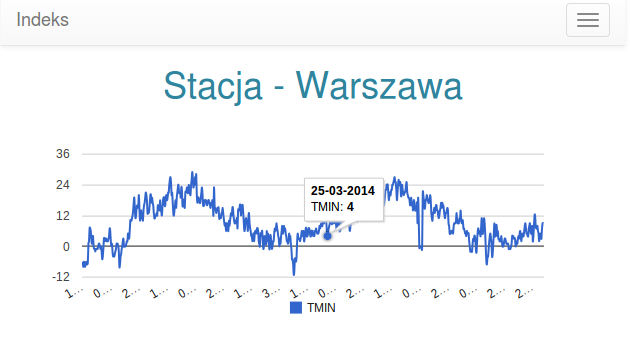
\includegraphics[width=\linewidth]{002}
	\caption{Wyrysowany wykres}
	\label{fig:wykres}
	\end{figure}
\subsection{Panel administracyjny}
Django automatycznie dostarcza panel administracyjny, który pozwala na wygodne zarządzanie danymi w bazie danych. Aby się do niego dostać należy z poziomu przeglądarki internetowej wejść na stronę internetową:
\begin{verbatim}
	http://127.0.0.1:8000/admin/
\end{verbatim}
oczywiście przy założeniu, że środowisko zostało już uruchomione. Następnie należy się zalogować. Po zalogowaniu ukaże się okno (Rysunek \ref{fig:panelAdmin}).
\begin{figure}[p]
	\centering
	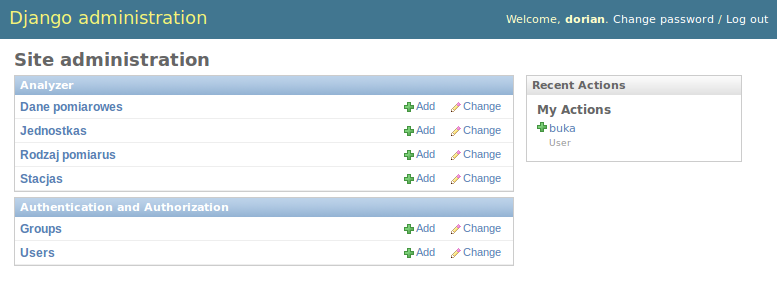
\includegraphics[width=\linewidth]{003}
	\caption{Panel administracyjny}
	\label{fig:panelAdmin}
	\end{figure}
\newline
W oknie tym można zarządzać tabelami oraz grupami użytkowników. 
W przypadku zarządzania użytkownikami można tworzyć, usuwać i zmieniać im uprawnienia. Przykładowo na rysunku \ref{fig:panelUzytkownicy} widać, że utworzony został nowy użytkownik o nazwie buka, ale nie otrzymał on prawa logowania się do panelu administracyjnego (nie została zaznaczona opcja \textit{staff status}). 
\begin{figure}[p]
	\centering
	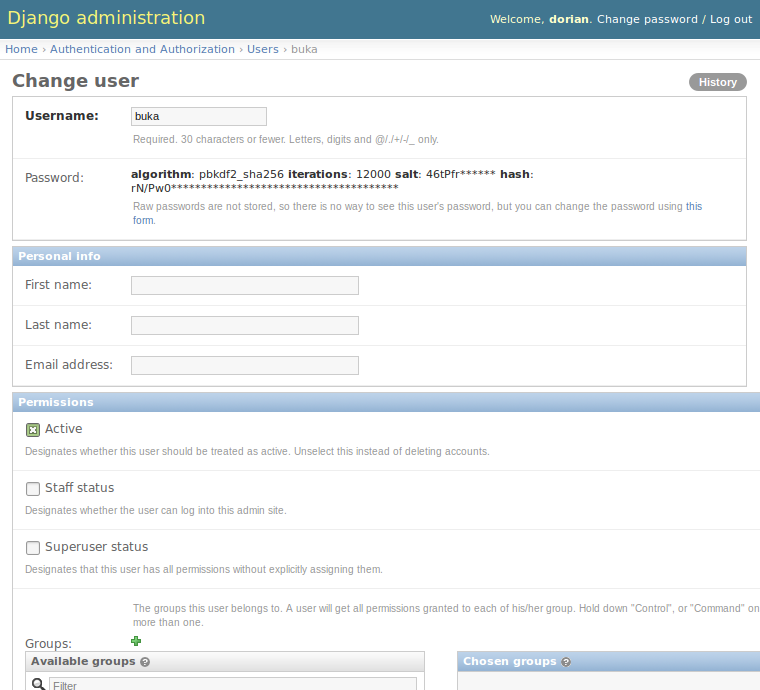
\includegraphics[width=\linewidth]{005}
	\caption{Panel Django - zmiana ustawień użytkownika}
	\label{fig:panelUzytkownicy}
	\end{figure}
\newline
Dodatkowo panel administracyjny pozwala na pełny dostęp do zawartości bazy - także można nawet usuwać lub dodawać pojedyncze rekordy. Na rysunku \ref{fig:panelPomiary} można zobaczyć fragment zestawienia zawartości tabeli \verb Analyzer_danepomiarowe . 
\begin{figure}[p]
	\centering
	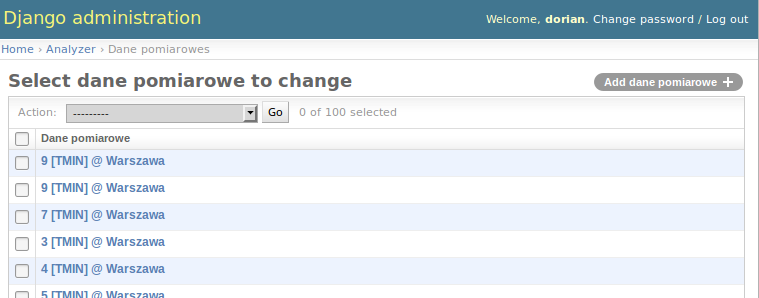
\includegraphics[width=\linewidth]{006}
	\caption{Panel Django - podgląd zawartości tabeli Analyzer\_danepomiarowe }
	\label{fig:panelPomiary}
	\end{figure}
\newline
Z tego zestawienia można wybrać jeden z pomiarów oraz go wyedytować. Edycję wpisu przedstawia rysunek \ref{fig:panelPomiar}.
\begin{figure}[p]
	\centering
	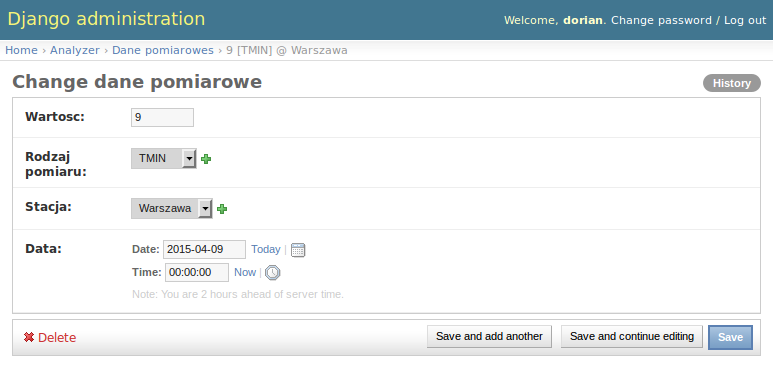
\includegraphics[width=\linewidth]{007}
	\caption{Panel Django - edycja wpisu tabeli Analyzer\_danepomiarowe }
	\label{fig:panelPomiar}
	\end{figure}
